\documentclass[../nirs.tex]{subfiles}
\usepackage{pdflscape}

\begin{document}
\section{Построение концептуальной и физической модели данных}
Концептуальная модель данных определяет смысловую структуру рассматриваемой
системы [\ref{ref:wiki-er-диаграммы}]. С ее помощью можно представить рассматриваемую предметную область
множеством сущностей и связей между ними. Каждая сущность обладает набором
свойств, именуемых атрибутами. Основная задача концептуальной модели -- передать
фундаментальное принципы и основные функциональные возможности проектируемой
системы [\ref{ref:wiki-er-диаграммы}].

Любая информационная система включает в себя некоторую систему управления базами
данных (СУБД). Концептуальная модель представления данных не подходит для
создания таблиц в реляционной СУБД. Чтобы можно было создать реляционную базу
данных необходимо концептуальную модель перевести в логическую, а затем в
физическую  модель данных, предназначенную для конкретной СУБД. На рисунке
\ref{fig:3_1_db_logical} представлена логическая модель данных разрабатываемой
системы.

\clearpage
\begin{landscape}

\begin{figure}[H]
	\centering
	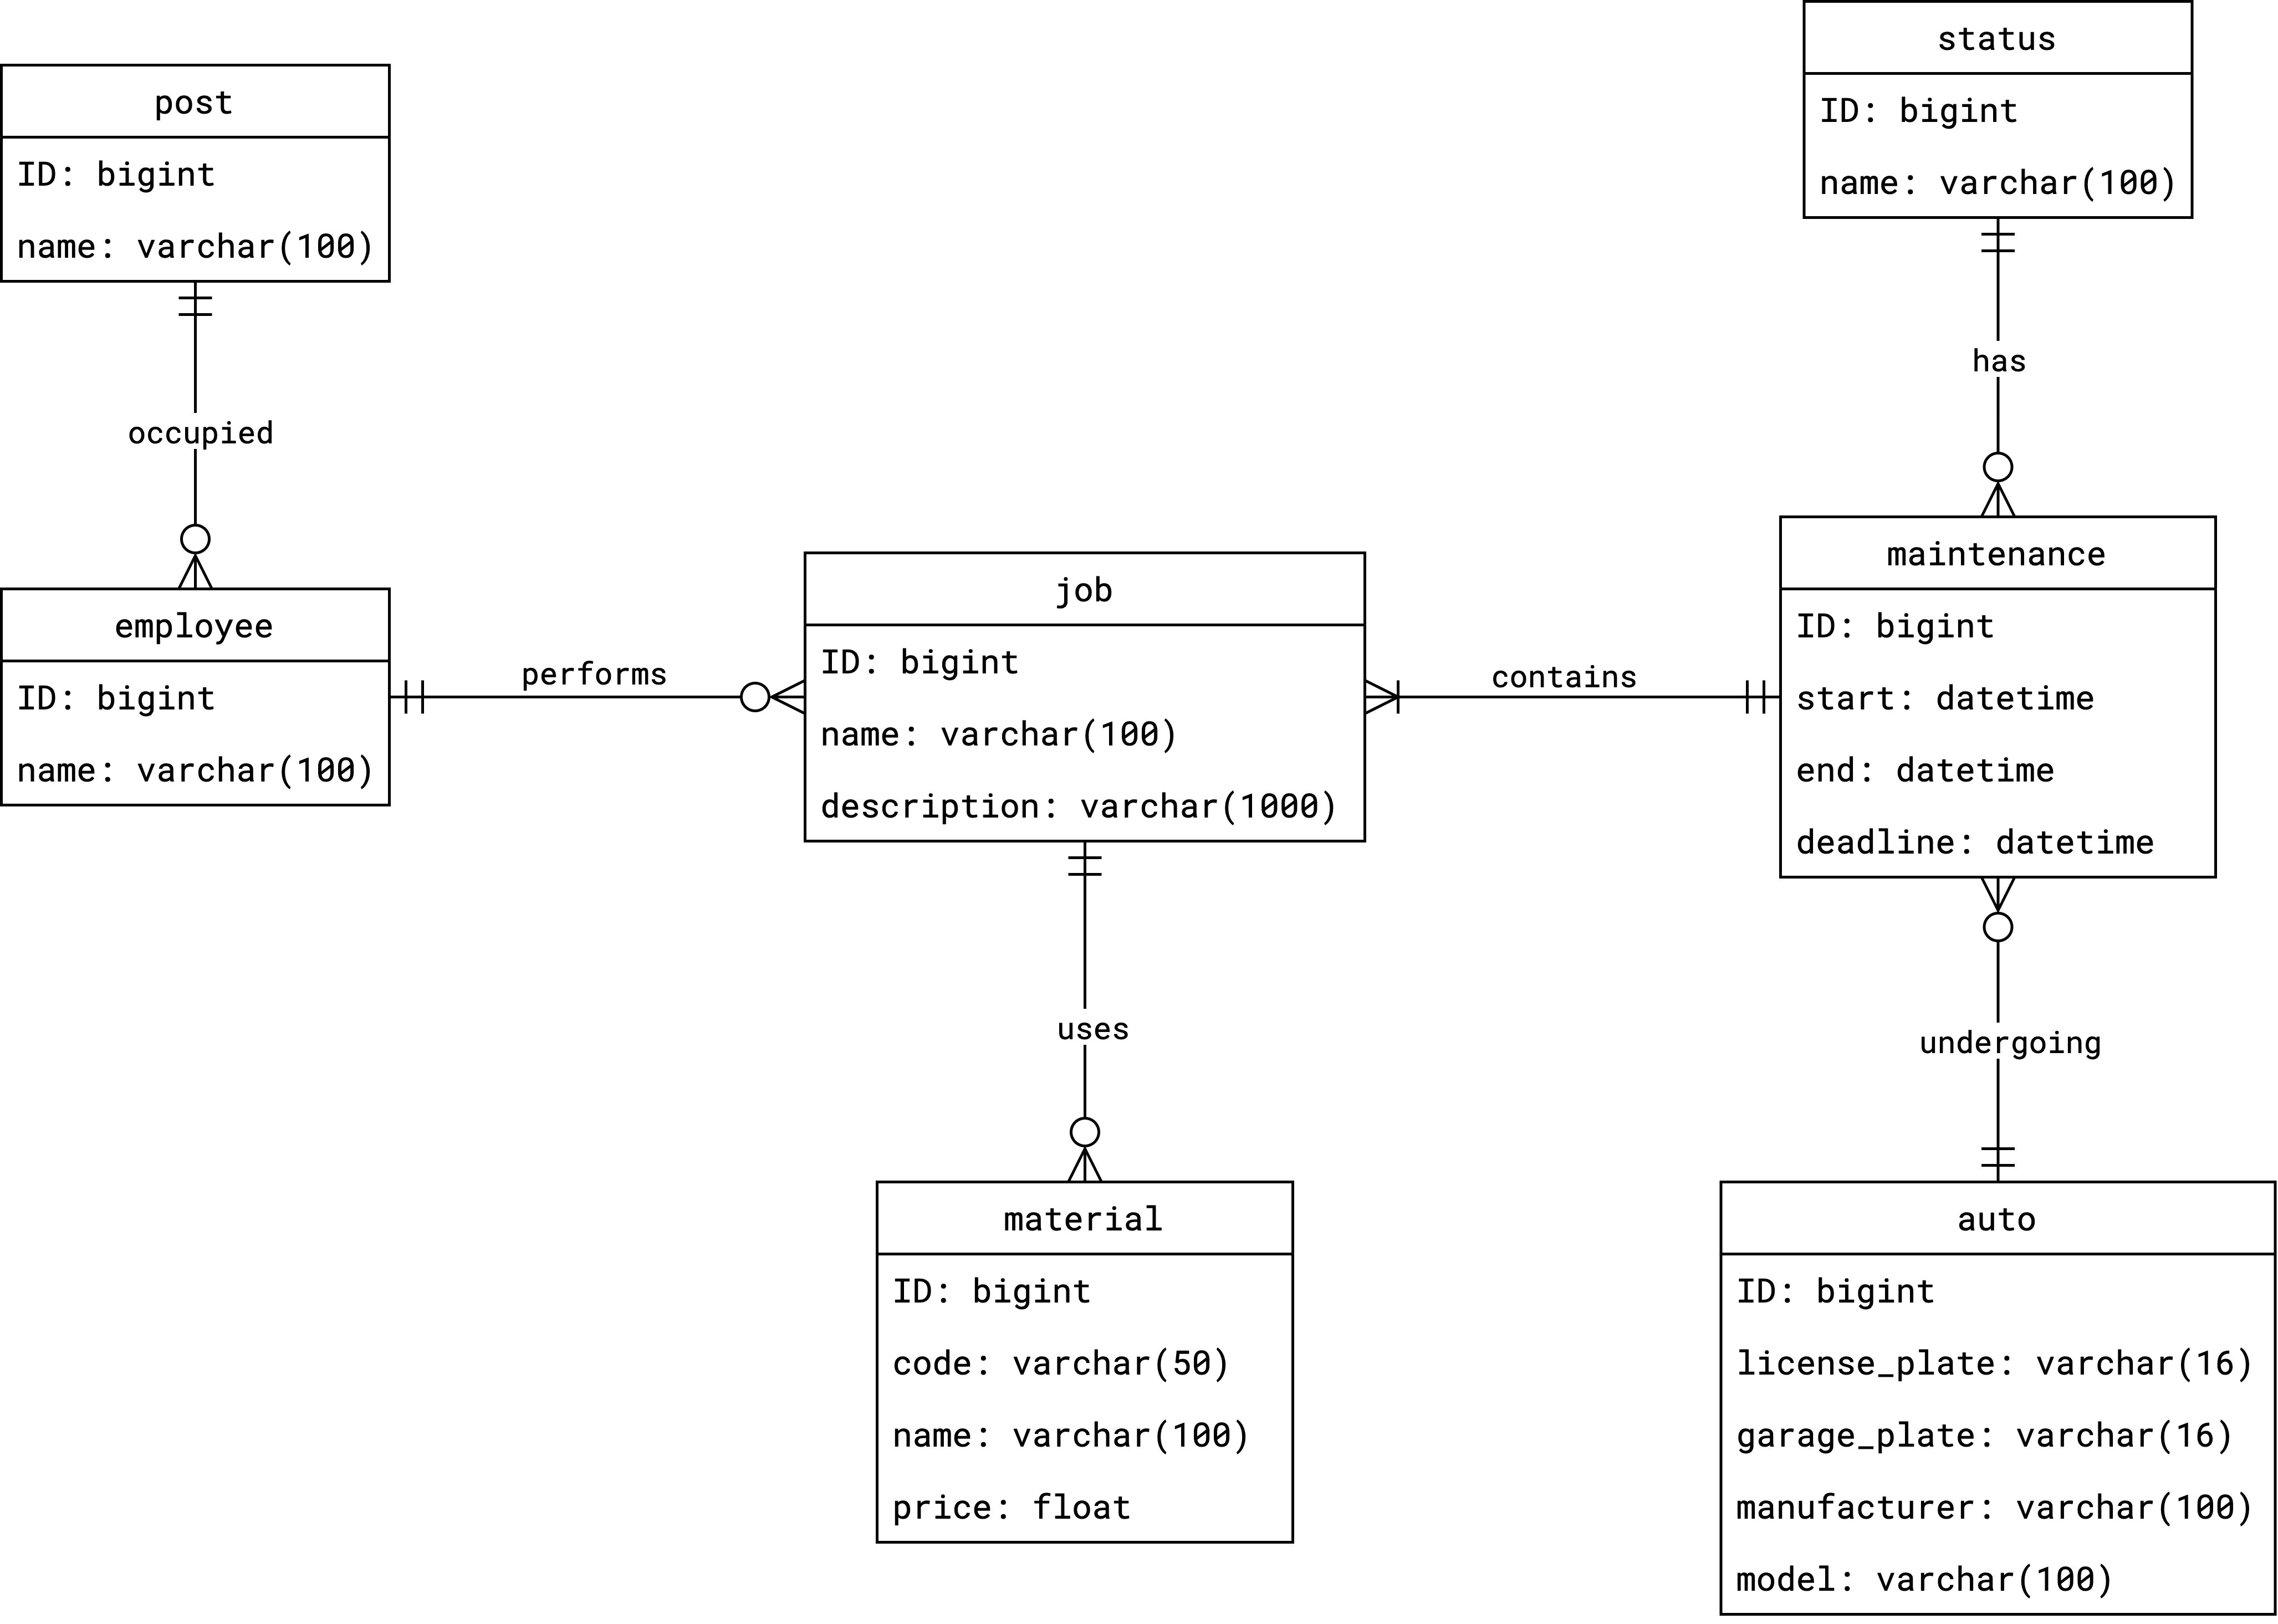
\includegraphics[keepaspectratio,width=\paperwidth]{./images/3_1_db_logical.png}
	\caption{Логическая модель данных разрабатываемой системы}
	\label{fig:3_1_db_logical}
\end{figure}

\end{landscape}
\clearpage

Спецификация сущностей приведена в таблицах \ref{tab:automobiles} --
\ref{tab:maintenance_mechanic}.
\begin{longtblr}
[
    caption = {
        Сущность
        \textquote{Автомобиль}
        (\texttt{\small automobiles})
    },
	label = {tab:automobiles},
]
{
	hlines, vlines,
	colspec = {L c c c},
	width = \textwidth,
	rowhead = 1,
	rowfoot = 0,
}
\SetCell[c=1,r=1]{c}{Код} & Тип & M & PK \\
    id & bigint & \checkmark & \checkmark \\
    registration\_plate & varchar & \checkmark & \\
    garage\_plate & varchar & \checkmark & \\
    vendor & varchar & \checkmark & \\
    model & varchar & \checkmark &
\end{longtblr}

\begin{longtblr}
[
    caption = {
        Сущность
        \textquote{Пользователь}
        (\texttt{\small users})
    },
	label = {tab:users},
]
{
	hlines, vlines,
	colspec = {L c c c},
	width = \textwidth,
	rowhead = 1,
	rowfoot = 0,
}
\SetCell[c=1,r=1]{c}{Код} & Тип & M & PK \\
    id & bigint & \checkmark & \checkmark \\
    full\_name & varchar & \checkmark & \\
    type & user\_type & \checkmark & \\
    login & varchar & \checkmark & \\
    password & char(512) & \checkmark &
\end{longtblr}

\begin{longtblr}
[
    caption = {
        Сущность
        \textquote{Материалы}
        (\texttt{\small materials})
    },
	label = {tab:materials},
]
{
	hlines, vlines,
	colspec = {L c c c},
	width = \textwidth,
	rowhead = 1,
	rowfoot = 0,
}
\SetCell[c=1,r=1]{c}{Код} & Тип & M & PK \\
    id & bigint & \checkmark & \checkmark \\
    name & varchar & \checkmark &
\end{longtblr}

\begin{longtblr}
[
    caption = {
        Сущность
        \textquote{Материалы автомобиля}
        (\texttt{\small auto\_materials})
    },
	label = {tab:auto_materials},
]
{
	hlines, vlines,
	colspec = {L c c c},
	width = \textwidth,
	rowhead = 1,
	rowfoot = 0,
}
\SetCell[c=1,r=1]{c}{Код} & Тип & M & PK \\
    id & bigint & \checkmark & \checkmark \\
    wear & float & \checkmark & \\
    material & bigint & \checkmark & \\
    auto & bigint & \checkmark &
\end{longtblr}

\begin{longtblr}
[
    caption = {
        Сущность
        \textquote{Склад материалов}
        (\texttt{\small storage})
    },
	label = {tab:storage},
]
{
	hlines, vlines,
	colspec = {L c c c},
	width = \textwidth,
	rowhead = 1,
	rowfoot = 0,
}
\SetCell[c=1,r=1]{c}{Код} & Тип & M & PK \\
    id & bigint & \checkmark & \checkmark \\
    quantity & float & \checkmark & \\
    material & bigint & \checkmark &
\end{longtblr}

\begin{longtblr}
[
    caption = {
        Сущность
        \textquote{Техническое обслуживание}
        (\texttt{\small maintenances})
    },
	label = {tab:maintenances},
]
{
	hlines, vlines,
	colspec = {L c c c},
	width = \textwidth,
	rowhead = 1,
	rowfoot = 0,
}
\SetCell[c=1,r=1]{c}{Код} & Тип & M & PK \\
    id & bigint & \checkmark & \checkmark \\
    status & maintenance\_status & \checkmark & \\
    start\_date & datetime & \checkmark & \\
    deadline & datetime & \checkmark & \\
    end\_date & datetime & \checkmark & \\
    auto & bigint & \checkmark &
\end{longtblr}

\begin{longtblr}
[
    caption = {
        Сущность
        \textquote{Работа ТО}
        (\texttt{\small maintenance\_works})
    },
	label = {tab:maintenance_works},
]
{
	hlines, vlines,
	colspec = {L c c c},
	width = \textwidth,
	rowhead = 1,
	rowfoot = 0,
}
\SetCell[c=1,r=1]{c}{Код} & Тип & M & PK \\
    id & bigint & \checkmark & \checkmark \\
    description & varchar & \checkmark & \\
    maintenance & bigint & \checkmark &
\end{longtblr}

\begin{longtblr}
[
    caption = {
        Сущность
        \textquote{Материалы ТО}
        (\texttt{\small maintenance\_work\_materials})
    },
	label = {tab:maintenance_work_materials},
]
{
	hlines, vlines,
	colspec = {L c c c},
	width = \textwidth,
	rowhead = 1,
	rowfoot = 0,
}
\SetCell[c=1,r=1]{c}{Код} & Тип & M & PK \\
    id & bigint & \checkmark & \checkmark \\
    planned\_waste & float & \checkmark &  \\
    real\_waste & float & \checkmark &  \\
    maintenance & bigint & \checkmark &  \\
    material & bigint & \checkmark &
\end{longtblr}

\begin{longtblr}
[
    caption = {
        Сущность
        \textquote{Исполнитель ТО}
        (\texttt{\small maintenance\_mechanic})
    },
	label = {tab:maintenance_mechanic},
]
{
	hlines, vlines,
	colspec = {L c c c},
	width = \textwidth,
	rowhead = 1,
	rowfoot = 0,
}
\SetCell[c=1,r=1]{c}{Код} & Тип & M & PK \\
    mechanic & bigint & \checkmark & \checkmark \\
    maintenance & bigint & \checkmark & \checkmark
\end{longtblr}


\end{document}
